\documentclass[12pt,a4paper,openany]{report}

\usepackage[T1]{fontenc}
\usepackage[utf8]{inputenc}
\usepackage[french]{babel}
\usepackage{lmodern}
\usepackage{microtype}
\usepackage[a4paper,top=2.5cm,bottom=2.5cm,left=3cm,right=2.5cm]{geometry}
\usepackage{setspace}
\usepackage{fancyhdr}
\usepackage{titlesec}
\usepackage{xcolor}
\usepackage{enumitem}
\usepackage{array}
\usepackage{booktabs}
\usepackage{graphicx}
\usepackage{float}
\usepackage[hidelinks]{hyperref}
\usepackage{tikz}
\usepackage{graphicx}
\usepackage{float}
\usetikzlibrary{positioning,arrows.meta,shapes.multipart}
\usepackage{url}
\usepackage[hidelinks]{hyperref}
\usepackage{amsmath}
\usepackage[utf8]{inputenc}
\usepackage[T1]{fontenc}
\usepackage[french]{babel}
\usepackage{amsmath}
\usepackage{tabularx}
\usepackage{array}
\usepackage{booktabs}
\usepackage[table]{xcolor}
\usepackage{tabularx}

\definecolor{ondaBlue}{RGB}{0,65,125}
\definecolor{ondaGray}{RGB}{90,90,90}

\onehalfspacing
\setlength{\parindent}{0.7cm}
\setlength{\parskip}{0.15em}

\setlist[itemize]{
  leftmargin=1.1cm,
  itemsep=0.25em,
  topsep=0.3em
}

\pagestyle{fancy}
\fancyhf{}
\fancyhead[L]{\small\textit{Rapport de PFA -- ONDA Badges Dakhla}}
\fancyhead[R]{\small\nouppercase{\leftmark}}
\fancyfoot[C]{\thepage}
\renewcommand{\headrulewidth}{0.4pt}
\renewcommand{\chaptermark}[1]{\markboth{#1}{}}

\titleformat{\chapter}[display]
  {\normalfont\bfseries\color{ondaBlue}}
  {\fontsize{22}{26}\selectfont\chaptertitlename~\thechapter}
  {0.4em}
  {\fontsize{29}{34}\selectfont}

\titlespacing*{\chapter}{0pt}{-10pt}{25pt}

\titleformat{\section}
  {\normalfont\Large\bfseries\color{ondaBlue}}
  {\thesection}{0.7em}{}

\titleformat{\subsection}
  {\normalfont\large\bfseries\color{ondaBlue}}
  {\thesubsection}{0.7em}{}

\addto\captionsfrench{%
  \renewcommand{\contentsname}{Table des matières}%
  \renewcommand{\listfigurename}{Table des figures}%
  \renewcommand{\figurename}{Figure}%
}

\newcommand{\frontchapter}[1]{%
  \chapter*{#1}%
  \addcontentsline{toc}{chapter}{#1}%
}

\newcommand{\logoPlaceholder}[1]{%
  \fbox{%
    \begin{minipage}[c][2.0cm][c]{4.2cm}
      \centering
      \color{ondaBlue}
      \small\bfseries
      #1
    \end{minipage}%
  }%
}

\newcommand{\figurePlaceholder}[2]{%
  \begin{figure}[H]
    \centering
    \fbox{%
      \begin{minipage}[c][4.2cm][c]{0.82\textwidth}
        \centering
        \color{ondaGray}
        \small
        \textit{Emplacement réservé pour une capture d'écran ou un schéma.}\\[0.4em]
        #1
      \end{minipage}%
    }
    \caption{#2}
  \end{figure}
}

\usepackage{fancyhdr}
\pagestyle{fancy}
\fancyhf{} % مسح جميع الإعدادات الافتراضية

% ضبط ارتفاع الهيدر باش يهز الشعارات بلا مشاكل
\setlength{\headheight}{35pt}

% الجهة ديال اليسار: نحطو فيها الشعارات
\fancyhead[L]{%
  
\includegraphics[height=1.0cm]{images/logo-fst-settat.png.png}%
  \hspace{0.2cm}%
  
\includegraphics[height=1.0cm]{images/logo-onda.png.png}%
}

% الجهة ديال اليمين: نحطو فيها عنوان الفصل أوتوماتيكياً
\fancyhead[R]{\leftmark}

% خط تحت الهيدر
\renewcommand{\headrulewidth}{0.5pt}

% أرقام الصفحات فـ الأسفل فـ الوسط
\fancyfoot[C]{\thepage}

\begin{document}

% ========================= PAGE DE GARDE =========================

\begin{titlepage}
  \thispagestyle{empty}

  % Remplacer ces cadres par les logos officiels.
  \noindent
  \begin{minipage}[t]{0.48\textwidth}
    \raggedright
     
\includegraphics[width=4.2cm]{images/logo-fst-settat.png}
   % \logoPlaceholder{LOGO\\FST SETTAT}
  \end{minipage}%
  \hfill
  \begin{minipage}[t]{0.48\textwidth}
    \raggedleft
     
\includegraphics[width=4.8cm]{images/logo-onda.png}
    %\logoPlaceholder{LOGO\\ONDA}
  \end{minipage}

  \vspace{1.0cm}

  \begin{center}
    {\large
    Université Hassan 1er\\[0.25em]
    Faculté des Sciences et Techniques de Settat\\[0.25em]
    Département Génie Informatique\\[1.1em]
    \textbf{Cycle d'Ingénieur en Informatique -- 1\textsuperscript{ère} année}}

    \vspace{1.5cm}

    {\Large\bfseries Rapport de Projet de Fin d'Année}

    \vspace{0.35cm}

    {\large Filière Génie Informatique}

    \vspace{1.0cm}

    \rule{0.88\textwidth}{0.7pt}

    \vspace{0.55cm}

    {\color{ondaBlue}
    \fontsize{21}{26}\selectfont
    \bfseries
     Conception et développement\\[0.2em]
    d'une application de gestion et de suivi des badges d'accès
    }

    \vspace{0.55cm}

    \rule{0.88\textwidth}{0.7pt}

    \vfill

  \begin{minipage}{0.88\textwidth}
    \begin{tabular}{@{}>{\raggedright\arraybackslash}p{0.55\textwidth} >{\raggedleft\arraybackslash}p{0.45\textwidth}@{}}
        \textbf{Réalisé par :} & \textbf{Encadré par :} \\[0.4cm]
        Oussama Tarchi & M. Hakim Bahir
    \end{tabular}
\end{minipage}

    \vspace{0.8cm}

    {\large
    Office National Des Aéroports (ONDA) -- Aéroport de Dakhla\\[0.25em]
    Service Technique Navigation}

    \vspace{0.5cm}

    {\large Année universitaire : 2025--2026}
  \end{center}
\end{titlepage}

\pagenumbering{arabic}

% ========================= REMERCIEMENTS =========================

\frontchapter{Remerciements}

Je tiens tout d'abord à exprimer ma profonde gratitude envers l'Office National
Des Aéroports (ONDA) pour m'avoir accueilli au sein de l'aéroport de Dakhla et
pour m'avoir donné l'occasion de réaliser ce projet dans un environnement
professionnel concret.

Je remercie chaleureusement mon encadrant professionnel, M. Hakim Bahir, pour
sa disponibilité, ses conseils avisés et le partage de son expérience tout au
long de ce projet.

Je remercie vivement l'ensemble du personnel de l'aéroport de Dakhla pour son
accueil, sa disponibilité et les explications fournies sur le fonctionnement du
suivi des badges d'accès. Ces échanges m'ont permis de mieux comprendre les
besoins opérationnels liés au renouvellement des badges et les enjeux de sûreté
associés au contrôle des accès.

Enfin, je remercie les professeurs de la Faculté des Sciences et Techniques de
Settat pour la qualité de la formation dispensée dans le Cycle d'Ingénieur en
Informatique, ainsi que pour les bases théoriques et méthodologiques mobilisées
au cours de ce projet.

% ========================= RÉSUMÉ =========================

\frontchapter{Résumé}

Ce rapport présente le travail réalisé dans le cadre d'un projet de fin d'année
effectué au sein de l'Office National Des Aéroports (ONDA), à l'aéroport de
Dakhla. Le projet porte sur la conception et le développement d'une application
de bureau destinée à améliorer la gestion et le suivi des badges d'accès.

L'application développée en Java permet d'importer un fichier Excel contenant
les informations relatives aux badges, d'identifier automatiquement les
colonnes utiles et de calculer la date d'expiration à partir de la date de
délivrance et de la durée prévue. Les badges sont ensuite classés selon leur
état : valide, nécessitant une relance ou expiré. Une interface graphique
Swing offre une visualisation centralisée, des filtres par état et un suivi
actualisé des données.

Le système intègre également des alertes locales persistantes, un mécanisme de
relance manuelle ou automatique par courrier électronique via SMTP, ainsi qu'un
historique JSON permettant d'éviter l'envoi de rappels en double au cours d'une
même journée. Cette solution contribue à réduire les opérations manuelles, à
améliorer la traçabilité du suivi et à limiter le risque de maintien d'un accès
avec un badge arrivé à expiration.

\vspace{0.5cm}
\noindent\rule{\linewidth}{0.4pt}

\vspace{0.2cm}
\noindent\textbf{Mots-clés :} Java, Swing, Apache POI, Excel, badges d'accès, expiration, notifications SMTP, ONDA, Dakhla.

\vspace{0.2cm}
\noindent\rule{\linewidth}{0.4pt}

% ========================= ABSTRACT =========================

\frontchapter{Abstract}

This report presents the work carried out during a final-year project at the
National Airports Authority of Morocco (ONDA), Dakhla Airport. The project
focuses on the design and development of a desktop application for managing and
monitoring airport access badges.

The Java application imports an Excel workbook containing badge records,
automatically identifies the relevant columns, and calculates the expiration
date from the delivery date and the planned duration. Badges are classified as
valid, requiring a reminder, or expired. A Swing graphical interface provides a
centralized view of the records, status-based filters, and refreshed monitoring
of the source data.

The solution also includes persistent local alerts, manual and automatic SMTP
email reminders, and a JSON history mechanism that prevents duplicate reminders
from being sent on the same day. The application therefore reduces manual
follow-up work, improves traceability, and helps prevent access badges from
remaining active after their expiration date.

\vspace{0.5cm}
\noindent\rule{\linewidth}{0.4pt}

\vspace{0.2cm}
\noindent\textbf{Keywords :} Java, Swing, Apache POI, Excel, access badges, expiration monitoring, SMTP notifications, ONDA, Dakhla.

\vspace{0.2cm}
\noindent\rule{\linewidth}{0.4pt}

% ========================= TABLES PRÉLIMINAIRES =========================

\cleardoublepage

\begingroup
\let\clearpage\relax
\let\cleardoublepage\relax
\tableofcontents
\vspace{1cm}
\listoffigures
\endgroup
% ========================= INTRODUCTION GÉNÉRALE =========================
\enlargethispage{\baselineskip}
\chapter*{Introduction générale}
\addcontentsline{toc}{chapter}{Introduction générale}

Dans un environnement aéroportuaire, la maîtrise des accès constitue un élément
essentiel pour assurer la sûreté des personnes, des infrastructures et des
opérations. Les badges d'accès délivrés aux agents, aux prestataires et aux
organismes partenaires sont accordés pour une durée déterminée. Leur expiration
doit donc être suivie avec rigueur afin d'éviter les retards de renouvellement,
les oublis administratifs ou toute situation pouvant entraîner un accès non
autorisé.

Au sein de l'aéroport de Dakhla, les informations relatives aux badges sont
regroupées dans un classeur Excel. La vérification manuelle des dates
d'expiration, l'identification des badges expirés ou proches de l'échéance et
l'envoi des relances deviennent répétitifs et exposés aux erreurs lorsque le
nombre d'enregistrements augmente.

Le projet \og ONDA Badges Dakhla \fg{} répond à ce besoin par le développement
d'une application desktop en Java permettant de lire le fichier Excel, de calculer
automatiquement les dates d'expiration, de visualiser l'état des badges et
d'envoyer des notifications par courrier électronique. L'application intègre aussi
un historique afin d'éviter les doublons et de garder une trace des alertes
effectuées.

Ce rapport présente les étapes de réalisation du projet et s'articule autour de
cinq chapitres :

\begin{enumerate}
    \item \textbf{Présentation de l'organisme d'accueil :}
    présentation de l'ONDA, de l'aéroport de Dakhla, du service d'accueil et du
    cadre général du stage.
    
    \item \textbf{Contexte général et analyse du besoin :}
    étude de la problématique, des objectifs du projet, des besoins fonctionnels
    et des contraintes à respecter.

    \item \textbf{Conception de la solution :}
    description de l'architecture retenue, du modèle de données, des composants
    principaux et des choix de conception.

    \item \textbf{Réalisation et mise en œuvre :}
    présentation de l'environnement de développement, des technologies utilisées,
    des interfaces et des fonctionnalités réalisées.

    \item \textbf{Tests, validation et perspectives :}
    présentation des essais effectués, des résultats obtenus, des limites de la
    solution et des améliorations envisageables.
\end{enumerate}

Enfin, une conclusion générale résume le travail réalisé, ses apports et les
perspectives d'amélioration.

% ========================= CHAPITRE 1 =========================

\chapter{Présentation de l'organisme d'accueil}

\section{Introduction}

Ce chapitre présente l'organisme dans lequel le projet a été réalisé, à savoir
l'Office National Des Aéroports, ainsi que le site d'accueil : l'aéroport de
Dakhla et son Service Technique Navigation. Il permet de situer l'application
dans son contexte professionnel et de comprendre l'importance du suivi des badges
d'accès dans un environnement aéroportuaire.

\section{L'Office National Des Aéroports (ONDA)}

L'Office National Des Aéroports est l'organisme marocain chargé de la gestion,
de l'exploitation, de l'entretien et du développement des aéroports civils
ouverts à la circulation aérienne publique. Dans ce cadre, l'ONDA contribue au
fonctionnement des infrastructures aéroportuaires et à la coordination des
services nécessaires à la sécurité et à la sûreté des opérations.

Les activités d'un aéroport reposent sur la collaboration de plusieurs
catégories d'agents et de prestataires. La délivrance de badges temporaires ou
permanents permet de contrôler l'accès aux zones autorisées. Le suivi de leur
validité s'inscrit ainsi dans une démarche de maîtrise des risques et de
traçabilité administrative.

\section{L'aéroport de Dakhla}

L'aéroport de Dakhla dessert la ville de Dakhla et accueille des activités
aériennes nécessitant la coordination de services opérationnels, techniques,
administratifs et de sûreté. Le contexte du site implique la circulation de
personnels appartenant à des organismes différents, ce qui explique la présence
de données telles que le nom du titulaire, son organisme, l'adresse électronique,
la date de délivrance et la durée prévue du badge.

\section{Le Service Technique Navigation et cadre du projet}

Ce stage a été réalisé au sein du Service Technique Navigation de l'aéroport de
Dakhla. Ce service intervient dans un environnement opérationnel où la rigueur,
la traçabilité et le respect des procédures sont essentiels au bon fonctionnement
des activités aéroportuaires.

Même si le service est principalement lié au suivi technique des équipements de
navigation aérienne, le contexte de travail implique également la circulation de
différents agents, prestataires et intervenants dans des zones réglementées. La
gestion des badges d'accès constitue donc un élément important pour assurer le
contrôle des autorisations et le respect des règles de sûreté.

Dans ce cadre, le projet \textit{ONDA Badges Dakhla} a été proposé afin de
faciliter le suivi des badges à partir du fichier Excel existant. L'application
permet d'exploiter les données déjà utilisées par le service, de calculer
automatiquement les dates d'expiration et de signaler les badges expirés ou
proches de l'échéance.

\section{Conclusion}

L'ONDA et l'aéroport de Dakhla constituent un cadre opérationnel dans lequel le
contrôle des autorisations d'accès doit être réalisé avec régularité. Le
chapitre suivant précise le fonctionnement existant, la problématique retenue
et les objectifs fonctionnels de l'application développée.

% ========================= CHAPITRE 2 =========================

\chapter{Contexte et cadrage du projet}

\section{Introduction}

Le cadrage du projet part d'un flux de données simple : un fichier Excel décrit
les badges délivrés, tandis que l'application doit transformer ces informations
en un suivi exploitable et en actions de relance. L'analyse porte donc sur les
données disponibles, les règles de calcul et les modes de notification.

\section{Analyse de l'existant}

Le classeur utilisé par le service contient une feuille dont l'intitulé est
« Liste Laissez-Passer 2026 ». Les premières lignes comprennent le titre puis
les en-têtes des colonnes. Les principales informations exploitées sont : le
numéro du badge, le nom et le prénom, l'adresse électronique, l'organisme, la
personne ou le service ayant délivré le badge, la date de délivrance et la durée
prévue.

Le système développé lit la première feuille du classeur avec la bibliothèque
Apache POI. La ligne d'en-tête est recherchée dynamiquement dans les quinze
premières lignes ; à défaut, la ligne 4 est utilisée comme position de repli.
Cette approche permet de tolérer de petites variations de présentation du
fichier sans modifier le code de l'application.

\begin{figure}[htbp]
    \centering
    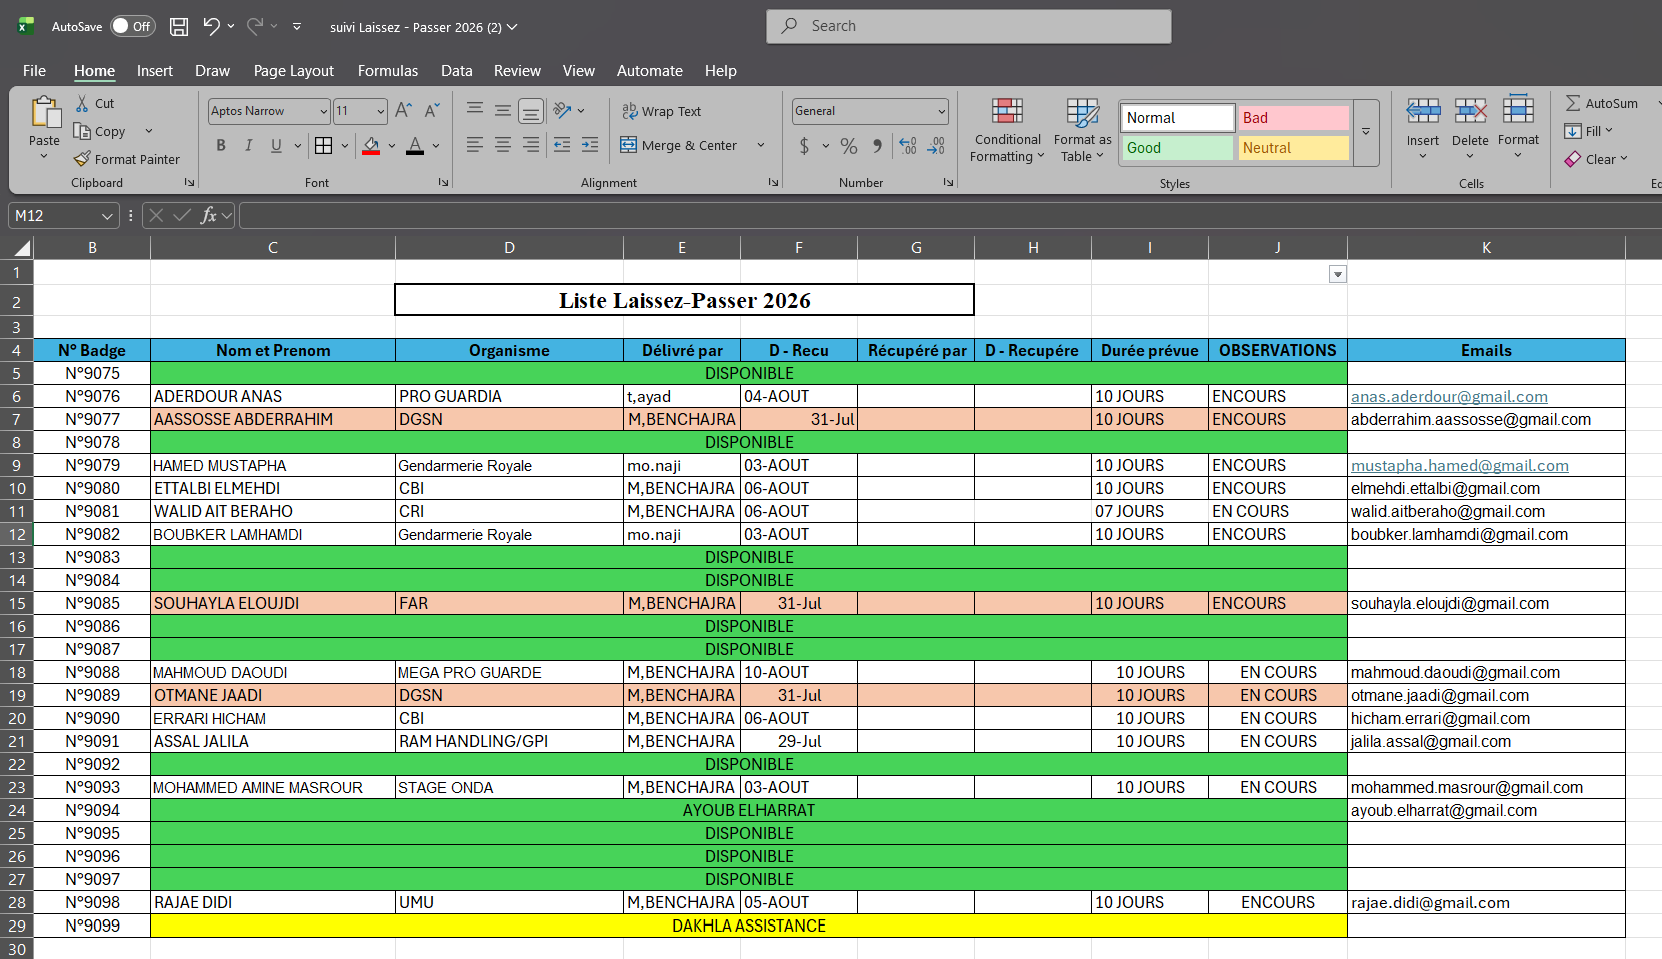
\includegraphics[width=0.8\textwidth]{images/Screenshot 2026-08-11 154740.png}
    \caption{Structure du fichier Excel exploité par l'application.}
\end{figure}
%\figurePlaceholder
%{Exemple de classeur source contenant les informations de délivrance et de durée des badges.}
%{Structure du fichier Excel exploité par l'application.}

\section{Problématique}

La problématique du projet peut être formulée de la manière suivante :

\begin{quote}
Comment gérer efficacement et automatiser le suivi des dates d'expiration des
badges du personnel de l'aéroport, simplifier le processus de renouvellement
et envoyer des notifications électroniques afin de prévenir les risques de
sécurité et les accès non autorisés, au moyen d'une application de bureau
centralisée ?
\end{quote}

\section{Objectifs du projet}

La solution vise principalement à :

\begin{itemize}
  \item importer les données d'un fichier Excel au format \texttt{.xlsx} ;
  \item calculer automatiquement la date d'expiration ;
  \item distinguer les badges valides, proches de l'expiration et expirés ;
  \item proposer une interface Swing centralisée avec filtres et indicateurs
        visuels ;
  \item afficher des alertes locales ;
  \item envoyer des rappels HTML par SMTP en mode manuel ou automatique ;
  \item conserver un historique JSON pour éviter les relances répétées.
\end{itemize}

\section{Principes fonctionnels retenus}

Pour chaque badge, l'échéance est calculée selon la règle suivante :

\{
\text{date d'expiration = date de délivrance + durée prévue en jours.}
\}

Le nombre de jours restants est ensuite comparé à un seuil configurable dans
l'interface. Un badge dont la date est dépassée est classé comme expiré. Un
badge dont l'échéance est comprise entre aujourd'hui et le seuil sélectionné
nécessite une relance. Les autres badges sont considérés comme valides.


%\figurePlaceholder
%{Tableau de bord Java Swing avec filtres, statuts colorés et panneau de relance.}
%{Vue fonctionnelle attendue du tableau de bord de suivi.}

\section{Conclusion}

Le cadrage met en évidence le rôle de l'application comme outil intermédiaire
entre le fichier Excel existant et les actions de suivi. Il conserve une source
de données familière tout en automatisant le calcul des échéances, la détection
des situations urgentes et la notification des personnes concernées.

% ========================= SQUELETTE DES CHAPITRES SUIVANTS =========================
% Les titres suivants enrichissent la table des matières sans ajouter de contenu
% inventé. Remplacer progressivement les textes indicatifs.
\chapter{Conception}

\section{Introduction}

Après l'étude de l'existant et la définition de la problématique, cette partie
présente la conception retenue pour l'application \textit{ONDA Badges Dakhla}.
L'objectif de cette conception est de transformer un besoin administratif réel
en une solution logicielle claire, fiable et simple à utiliser par le service
concerné.

La solution conçue est une application bureautique Java permettant de lire le
fichier Excel utilisé pour le suivi des laissez-passer, de calculer
automatiquement les dates d'expiration, de classer les badges selon leur niveau
d'urgence et de déclencher des alertes locales ou des relances par courrier
électronique. Le choix d'une application desktop se justifie par le contexte de
travail : les données sont déjà centralisées dans un fichier Excel local, les
agents utilisent un poste Windows, et le besoin principal est d'automatiser le
contrôle sans imposer une infrastructure serveur ou une base de données.

La conception a donc été orientée vers trois principes : automatiser les tâches
répétitives, conserver une interface lisible pour l'utilisateur, et assurer une
traçabilité minimale des alertes et des courriels envoyés.

\section{Spécifications fonctionnelles}

Les spécifications fonctionnelles décrivent les services que l'application doit
fournir à l'utilisateur final. Dans ce projet, l'utilisateur principal est
l'agent chargé du suivi des badges ou toute personne du service habilitée à
contrôler les échéances des laissez-passer.

\begin{table}[H]
\centering
\small
\renewcommand{\arraystretch}{1.5} % A nice comfortable row height
\arrayrulecolor{ondaBlue} % Colors the borders/edges to match your theme
\setlength{\arrayrulewidth}{1pt} % Makes the edges slightly thicker and crisper

% The "|" symbols create the vertical edges
\begin{tabularx}{\textwidth}{|>{\raggedright\arraybackslash\bfseries}p{0.25\textwidth}|>{\raggedright\arraybackslash}X|}
\hline
% Header row with dark blue background and white text
\rowcolor{ondaBlue} 
\textcolor{white}{\textbf{Besoin}} & \textcolor{white}{\textbf{Description fonctionnelle}} \\
\hline

% Row 1 - Light tinted background
\rowcolor{ondaBlue!5} 
Importer les données & Charger un fichier Excel contenant la liste des badges et extraire automatiquement les informations nécessaires. \\
\hline

% Row 2 - White background
Calculer les échéances & Déterminer la date d'expiration à partir de la date de délivrance et de la durée prévue. \\
\hline

% Row 3 - Light tinted background
\rowcolor{ondaBlue!5} 
Visualiser les badges & Afficher les badges dans un tableau lisible, avec les informations essentielles et un statut visuel. \\
\hline

% Row 4 - White background
Filtrer les urgences & Permettre l'affichage des badges expirés, des badges à relancer ou de l'ensemble des badges. \\
\hline

% Row 5 - Light tinted background
\rowcolor{ondaBlue!5} 
Notifier localement & Afficher une alerte persistante lorsqu'un badge expiré ou proche de l'expiration est détecté. \\
\hline

% Row 6 - White background
Envoyer les relances & Générer et envoyer des e-mails HTML aux détenteurs des badges concernés. \\
\hline

% Row 7 - Light tinted background
\rowcolor{ondaBlue!5} 
Éviter les doublons & Mémoriser les alertes consultées et les e-mails déjà envoyés afin d'éviter les répétitions inutiles. \\
\hline

\end{tabularx}
\caption{Synthèse des besoins fonctionnels de l'application}
\label{tab:besoins-fonctionnels}
\end{table}

\subsection{Importation et lecture du fichier Excel}

Le fichier Excel constitue la source principale des données. L'application doit
permettre à l'utilisateur de sélectionner ce fichier depuis l'interface graphique
et de mémoriser le chemin choisi pour les utilisations suivantes. Le fichier
attendu correspond à la liste des laissez-passer, contenant notamment le numéro
du badge, le nom du détenteur, son e-mail, son organisme, la date de délivrance
et la durée prévue.

La conception ne repose pas sur une position figée des colonnes uniquement.
Même si le format standard place les en-têtes à la quatrième ligne du fichier,
le service de lecture doit être capable de détecter dynamiquement la ligne
d'en-tête dans les premières lignes du classeur.

\begin{table}[H]
\centering
\small
\renewcommand{\arraystretch}{1.5} % Espacement vertical aéré
\arrayrulecolor{ondaBlue} % Bords aux couleurs de votre thème
\setlength{\arrayrulewidth}{1pt} % Épaisseur des bordures

\begin{tabularx}{\textwidth}{|>{\raggedright\arraybackslash\bfseries}p{0.25\textwidth}|>{\raggedright\arraybackslash}X|}
\hline
% En-tête avec fond bleu et texte en blanc
\rowcolor{ondaBlue} 
\textcolor{white}{\textbf{Champ}} & \textcolor{white}{\textbf{Utilisation dans l'application}} \\
\hline

% Ligne 1 - Fond légèrement teinté
\rowcolor{ondaBlue!5} 
N\textsuperscript{o} Badge & Identifiant principal du laissez-passer. \\
\hline

% Ligne 2 - Fond blanc
Nom et Prénom & Identification du détenteur du badge. \\
\hline

% Ligne 3 - Fond légèrement teinté
\rowcolor{ondaBlue!5} 
Email & Adresse utilisée pour l'envoi des relances automatiques. \\
\hline

% Ligne 4 - Fond blanc
Organisme & Société, organisme ou service auquel appartient le détenteur. \\
\hline

% Ligne 5 - Fond légèrement teinté
\rowcolor{ondaBlue!5} 
Délivré par & Information de suivi sur l'autorité ou l'agent de délivrance. \\
\hline

% Ligne 6 - Fond blanc
D-délivrance & Date de départ pour le calcul de l'échéance. \\
\hline

% Ligne 7 - Fond légèrement teinté
\rowcolor{ondaBlue!5} 
Durée prévue & Nombre de jours à ajouter à la date de délivrance. \\
\hline

\end{tabularx}
\caption{Champs Excel exploités par la solution}
\label{tab:champs-excel} % Ajout d'un label pour pouvoir référencer la table dans le texte
\end{table}

\subsection{Calcul de la date d'expiration}

La date d'expiration n'est pas saisie manuellement par l'utilisateur dans
l'application. Elle est calculée automatiquement afin de limiter les erreurs et
d'assurer une règle uniforme pour tous les badges. La règle métier principale
est la suivante :

\[
\text{Date d'expiration} = \text{Date de délivrance} + \text{Durée prévue en jours}
\]

Par exemple, si un badge est délivré le 18/07/2026 avec une durée prévue de 10
jours, l'application calcule une expiration au 28/07/2026. Cette règle permet de
transformer des informations brutes issues du tableau Excel en indicateurs
directement exploitables par l'agent.

Le calcul tient compte de plusieurs formats de dates, notamment les dates Excel
natives, les formats numériques classiques et les mois écrits en français comme
\textit{juil}, \textit{août} ou \textit{déc}. La durée prévue est interprétée
comme un nombre de jours : une valeur comme \textit{15 JOURS} ou \textit{15}
donne donc le même résultat fonctionnel.

\subsection{Visualisation et filtrage des badges}

L'interface principale est conçue comme un tableau de bord. Elle regroupe les
paramètres de configuration, le choix du fichier Excel, les options de relance
et une zone de visualisation des badges. Le tableau affiche uniquement les
informations nécessaires à la prise de décision : numéro du badge, nom et
prénom, organisme, e-mail, date d'expiration et statut.

Trois vues de filtrage sont prévues :

\begin{itemize}
  \item \textbf{Tous} : affiche l'ensemble des badges chargés depuis le fichier
  Excel.
  \item \textbf{À relancer} : affiche les badges dont l'expiration est comprise
  entre la date du jour et le délai de rappel sélectionné.
  \item \textbf{Expirés} : affiche les badges dont la date d'expiration est déjà
  dépassée.
\end{itemize}

Le délai de rappel est configurable par l'utilisateur. Les valeurs proposées
sont 1, 3, 7, 14 et 30 jours. Ce choix permet d'adapter le suivi au niveau
d'anticipation souhaité par le service.

\begin{table}[H]
\centering
\small
\renewcommand{\arraystretch}{1.5} % Espacement vertical aéré
\arrayrulecolor{ondaBlue} % Bords aux couleurs de votre thème
\setlength{\arrayrulewidth}{1pt} % Épaisseur des bordures

% Configuration pour 3 colonnes : 20% pour Cas, 30% pour Condition, et le reste (X) pour Interprétation
\begin{tabularx}{\textwidth}{|>{\raggedright\arraybackslash\bfseries}p{0.20\textwidth}|>{\raggedright\arraybackslash}p{0.30\textwidth}|>{\raggedright\arraybackslash}X|}
\hline
% En-tête avec fond bleu et texte en blanc
\rowcolor{ondaBlue} 
\textcolor{white}{\textbf{Cas}} & \textcolor{white}{\textbf{Condition}} & \textcolor{white}{\textbf{Interprétation}} \\
\hline

% Ligne 1 - Fond légèrement teinté
\rowcolor{ondaBlue!5} 
Expiré & Jours restants $< 0$ & Le badge n'est plus valide et nécessite une action immédiate. \\
\hline

% Ligne 2 - Fond blanc
À relancer & $0 \leq$ jours restants $\leq$ délai choisi & Le badge est encore valide, mais son renouvellement doit être anticipé. \\
\hline

% Ligne 3 - Fond légèrement teinté
\rowcolor{ondaBlue!5} 
Valide & Jours restants $>$ délai choisi & Aucun traitement urgent n'est nécessaire. \\
\hline

\end{tabularx}
\caption{Règles de classification des badges}
\label{tab:regles-classification}
\end{table}

\subsection{Alertes locales et relances par courrier électronique}

La solution distingue deux types d'alertes complémentaires.

Le premier type est l'alerte locale. Lorsqu'un badge expiré ou proche de
l'expiration est détecté, l'application affiche une fenêtre d'alerte persistante
dans l'environnement Windows. Cette alerte attire l'attention de l'utilisateur
sans nécessiter l'ouverture permanente du fichier Excel. Pour éviter que la même
alerte ne soit affichée à chaque rafraîchissement, les badges déjà consultés
sont enregistrés dans le fichier local \texttt{seen\_badges.json}.

Le second type est la relance par e-mail. L'application prépare un message HTML
en français contenant les informations essentielles du badge : numéro, nom du
détenteur, organisme, date d'expiration et date du jour. Le message est envoyé
via un serveur SMTP configuré depuis l'interface.

\subsection{Modes manuel et automatique}

Deux modes d'exécution ont été prévus.

En mode manuel, l'utilisateur clique sur le bouton \textit{LANCER} après avoir
vérifié le fichier, le délai de rappel et les paramètres SMTP. Ce mode donne un
contrôle direct à l'agent et convient particulièrement aux tests, aux envois
ponctuels ou aux situations nécessitant une validation humaine.

En mode automatique, l'application planifie l'envoi quotidien des relances à
09h00. Ce mode réduit le risque d'oubli et transforme le suivi des badges en un
processus régulier. Le bouton d'envoi manuel est désactivé lorsque ce mode est
actif, afin de rendre l'état de l'application plus clair pour l'utilisateur.

En parallèle, un mécanisme de surveillance vérifie périodiquement la date de
modification du fichier Excel. Si le fichier est modifié, les données sont
rechargées et les alertes locales sont recalculées.

\subsection{Traçabilité et prévention des doublons}

La traçabilité est un point important dans une application de relance. Sans
mécanisme de suivi, un même détenteur pourrait recevoir plusieurs fois le même
message dans la même journée, ou une même alerte pourrait réapparaître à chaque
ouverture.

La conception prévoit donc deux fichiers d'historique :

\begin{itemize}
  \item \texttt{seen\_badges.json} pour mémoriser les badges déjà affichés dans
  les alertes locales ;
  \item \texttt{sent\_emails\_history.json} pour mémoriser les relances e-mail
  déjà envoyées.
\end{itemize}

L'identification d'une alerte locale repose sur une clé composée du numéro de
badge et de sa date d'expiration. Ainsi, si un badge est renouvelé et que sa date
d'expiration change, il peut de nouveau être signalé. Pour les e-mails, le
système compare le numéro du badge, la date d'expiration et la date d'envoi afin
d'empêcher les doublons le même jour.

\section{Diagramme de classes}

Le diagramme de classes présente les principales classes de l'application
ONDA Badges Dakhla ainsi que leurs responsabilités et leurs relations.
L'organisation retenue sépare l'interface graphique, le contrôle, les services
métier et le modèle de données.

\begin{figure}[H]
\centering

\resizebox{\textwidth}{!}{%
\begin{tikzpicture}[
    class/.style={
        rectangle split,
        rectangle split parts=3,
        rectangle split part fill={ondaBlue!15,white,white},
        draw=ondaBlue,
        thick,
        rounded corners=2pt, 
        text width=4.6cm, % Enlarged to ensure methods like requiresRelance() fit perfectly
        font=\scriptsize,
        align=left,
        inner sep=5pt % Slightly increased padding
    },
    relation/.style={
        -{Latex[length=2.5mm]},
        thick,
        draw=ondaGray
    },
    dependency/.style={
        -{Latex[length=2.5mm]},
        thick,
        dashed,
        draw=ondaGray
    },
    % New style for relationship names so they don't block the arrows
    relLabel/.style={
        font=\scriptsize\itshape,
        text=black
    },
    % Styles for Multiplicities (1, *)
    mult1/.style={
        font=\tiny,
        text=darkgray,
        pos=0.1 % Near the start of the arrow
    },
    mult2/.style={
        font=\tiny,
        text=darkgray,
        pos=0.9 % Near the end of the arrow
    }
]

% =========================================================
% Classes principales (Spaced out in a larger grid)
% =========================================================

% --- Colonne Centrale (Interface & Contrôle) ---
\node[class] (app) at (0,12) {
    \centering\textbf{\texttt{App}}
    \nodepart{second}
    -- aucun attribut principal
    \nodepart{third}
    + \texttt{main(args)}\\
    + \texttt{lockInstance()}\\
    + \texttt{setupSystemTray()}
};

\node[class] (dashboard) at (0,7.5) {
    \centering\textbf{\texttt{MainDashboardFrame}}
    \nodepart{second}
    - \texttt{masterBadgeList}\\
    - \texttt{currentFilteredList}\\
    - \texttt{excelPathField}
    \nodepart{third}
    + \texttt{chargerFichierExcel()}\\
    + \texttt{appliquerFiltre()}\\
    + \texttt{lancerRelance()}\\
    + \texttt{afficherHistorique()}
};

\node[class] (controller) at (0,3) {
    \centering\textbf{\texttt{BadgeController}}
    \nodepart{second}
    - \texttt{excelParserService}\\
    - \texttt{notificationService}
    \nodepart{third}
    + \texttt{loadBadgesFromExcel()}\\
    + \texttt{filterBadges()}
};

\node[class] (notification) at (0,-1.5) {
    \centering\textbf{\texttt{NotificationService}}
    \nodepart{second}
    - \texttt{seenBadgesFile}
    \nodepart{third}
    + \texttt{notifyExpiredBadges()}\\
    + \texttt{loadSeenBadges()}\\
    + \texttt{saveSeenBadges()}
};

\node[class] (dialog) at (0,-6) {
    \centering\textbf{\texttt{CustomNotificationDialog}}
    \nodepart{second}
    - \texttt{expiredBadges}\\
    - \texttt{warningBadges}
    \nodepart{third}
    + \texttt{setVisible()}\\
    + \texttt{fermerAlerte()}
};


% --- Colonne Droite (Services & Tâches de fond) ---
\node[class] (daemon) at (7.5,12) {
    \centering\textbf{\texttt{ScheduledRelanceDaemon}}
    \nodepart{second}
    - \texttt{excelFilePath}\\
    - \texttt{scheduler}\\
    - \texttt{emailScheduler}
    \nodepart{third}
    + \texttt{start()}\\
    + \texttt{stop()}\\
    + \texttt{startEmailScheduler()}
};

\node[class] (email) at (7.5,7.5) {
    \centering\textbf{\texttt{EmailService}}
    \nodepart{second}
    - \texttt{smtpHost}\\
    - \texttt{smtpPort}\\
    - \texttt{senderEmail}\\
    - \texttt{historyManager}
    \nodepart{third}
    + \texttt{sendBulkReminders()}\\
    + \texttt{isNetworkAvailable()}
};

\node[class] (history) at (7.5,3) {
    \centering\textbf{\texttt{EmailHistoryManager}}
    \nodepart{second}
    - \texttt{historyFile}\\
    - \texttt{historyRecords}
    \nodepart{third}
    + \texttt{isAlreadySentToday()}\\
    + \texttt{recordSentEmail()}\\
    + \texttt{loadHistory()}\\
    + \texttt{saveHistory()}
};


% --- Colonne Gauche (Traitement & Modèle de Données) ---
\node[class] (parser) at (-7.5,3) {
    \centering\textbf{\texttt{ExcelParserService}}
    \nodepart{second}
    - \texttt{columnMap}\\
    - \texttt{dateFormatters}
    \nodepart{third}
    + \texttt{parseExcelFile()}\\
    + \texttt{parseExcelStream()}
};

\node[class] (badge) at (-7.5,-1.5) {
    \centering\textbf{\texttt{Badge}}
    \nodepart{second}
    - \texttt{badgeNumber}\\
    - \texttt{fullName}\\
    - \texttt{email}\\
    - \texttt{organisme}\\
    - \texttt{deliveryDate}\\
    - \texttt{calculatedExpiration}
    \nodepart{third}
    + \texttt{getDaysRemaining()}\\
    + \texttt{getStatus()}\\
    + \texttt{requiresRelance()}
};

\node[class] (status) at (-7.5,-6) {
    \centering\textbf{\texttt{BadgeStatus}}
    \nodepart{second}
    \texttt{EXPIRED}\\
    \texttt{WARNING\_RELANCE}\\
    \texttt{VALID}
    \nodepart{third}
    Énumération représentant\\
    l'état du badge
};

% =========================================================
% Relations (With Multiplicities and Clean Labels)
% =========================================================

% Horizontales
\draw[relation] (app.east) -- (daemon.west) 
    node[mult1, above] {1} node[mult2, above] {1}
    node[midway, above=3pt, relLabel] {planifie};

\draw[relation] (dashboard.east) -- (email.west) 
    node[mult1, above] {1} node[mult2, above] {1}
    node[midway, above=3pt, relLabel] {déclenche};

\draw[relation] (controller.west) -- (parser.east) 
    node[mult1, above] {1} node[mult2, above] {1}
    node[midway, above=3pt, relLabel] {lit};

% Verticales - Centre
\draw[relation] (app.south) -- (dashboard.north) 
    node[mult1, right] {1} node[mult2, right] {1}
    node[midway, right=3pt, relLabel] {initialise};

\draw[relation] (dashboard.south) -- (controller.north) 
    node[mult1, right] {1} node[mult2, right] {1}
    node[midway, right=3pt, relLabel] {utilise};

\draw[relation] (controller.south) -- (notification.north) 
    node[mult1, right] {1} node[mult2, right] {1}
    node[midway, right=3pt, relLabel] {notifie};

\draw[relation] (notification.south) -- (dialog.north) 
    node[mult1, right] {1} node[mult2, right] {*}
    node[midway, right=3pt, relLabel] {affiche};

% Verticales - Droite
\draw[relation] (daemon.south) -- (email.north) 
    node[mult1, right] {1} node[mult2, right] {1}
    node[midway, right=3pt, relLabel] {utilise};

\draw[relation] (email.south) -- (history.north) 
    node[mult1, right] {1} node[mult2, right] {1}
    node[midway, right=3pt, relLabel] {consulte};

% Verticales - Gauche
\draw[relation] (parser.south) -- (badge.north) 
    node[mult1, left] {1} node[mult2, left] {*}
    node[midway, left=3pt, relLabel] {crée};

\draw[dependency] (badge.south) -- (status.north) 
    node[mult1, left] {*} node[mult2, left] {1}
    node[midway, left=3pt, relLabel] {retourne};

\end{tikzpicture}%
}

\caption{Diagramme de classes organisé de l'application ONDA Badges Dakhla}
\label{fig:diagramme-classes}
\end{figure}

\section{Conception de l'interface utilisateur}

L'interface a été pensée pour un usage administratif quotidien : elle doit être
directe, lisible et suffisamment dense pour permettre un contrôle rapide des
données. La fenêtre principale est divisée en plusieurs zones.

Le bandeau supérieur affiche l'identité de l'application avec le logo ONDA, le
titre \textit{ONDA Badges Dakhla -- Application de Relance Automatique} et un
bouton \textit{Historique}. Ce bouton ouvre un journal séparé contenant deux
onglets : les badges déjà vus et les e-mails envoyés.

Le panneau de configuration SMTP regroupe les paramètres nécessaires à l'envoi
des courriels : serveur, port, adresse expéditeur et mot de passe. Le panneau de
source d'entrée permet de sélectionner le fichier Excel. Le panneau
\textit{Configuration \& Exécution} contient le délai de rappel, le choix du mode
manuel ou automatique, ainsi que le bouton de lancement.

Enfin, la zone de visualisation présente les badges sous forme de tableau. Les
lignes sont colorées selon leur état : rouge pour les badges expirés, jaune pour
les badges à relancer et vert pour les badges valides. Cette représentation
permet à l'utilisateur d'identifier immédiatement les priorités.

\section{Conception de la persistance locale}

La solution ne nécessite pas de base de données. Les données opérationnelles
proviennent du fichier Excel, tandis que les préférences et les historiques sont
stockés localement.

\begin{table}[H]
\centering
\small
\renewcommand{\arraystretch}{1.5}
\arrayrulecolor{ondaBlue}
\setlength{\arrayrulewidth}{1pt}

\begin{tabularx}{\textwidth}{|>{\raggedright\arraybackslash\bfseries}p{0.32\textwidth}|>{\raggedright\arraybackslash}X|}
\hline
\rowcolor{ondaBlue} 
\textcolor{white}{\textbf{Fichier}} & \textcolor{white}{\textbf{Rôle}} \\
\hline

\rowcolor{ondaBlue!5} 
\texttt{application.properties} & Contient les valeurs par défaut de l'application, notamment le nom de l'application et le chemin Excel par défaut. \\
\hline

\texttt{config.properties} & Conserve les paramètres choisis par l'utilisateur : chemin du fichier Excel, serveur SMTP, port, e-mail expéditeur et mot de passe. \\
\hline

\rowcolor{ondaBlue!5} 
\texttt{seen\_badges.json} & Mémorise les alertes locales déjà consultées afin de ne pas afficher plusieurs fois la même alerte. \\
\hline

\texttt{sent\_emails\_history.json} & Conserve l'historique des relances envoyées et permet d'éviter un nouvel envoi identique le même jour. \\
\hline

\end{tabularx}
\caption{Fichiers de configuration et de persistance locale}
\label{tab:fichiers-config}
\end{table}

\section{Choix technologiques}

Les choix technologiques ont été faits en fonction des contraintes du projet :
application locale, manipulation d'un fichier Excel, interface simple et envoi
d'e-mails.

\begin{table}[H]
\centering
\small
\renewcommand{\arraystretch}{1.5}
\arrayrulecolor{ondaBlue}
\setlength{\arrayrulewidth}{1pt}

\begin{tabularx}{\textwidth}{|>{\raggedright\arraybackslash\bfseries}p{0.25\textwidth}|>{\raggedright\arraybackslash}X|}
\hline
\rowcolor{ondaBlue} 
\textcolor{white}{\textbf{Technologie}} & \textcolor{white}{\textbf{Justification}} \\
\hline

\rowcolor{ondaBlue!5} 
Java 17 & Version moderne et stable du langage Java, adaptée aux applications desktop et à l'organisation en classes métiers. \\
\hline

Swing / AWT & Bibliothèques natives Java permettant de créer une interface bureautique, des boîtes de dialogue, une table et une icône système. \\
\hline

\rowcolor{ondaBlue!5} 
FlatLaf & Améliore l'apparence de Swing avec un rendu plus moderne et plus confortable pour l'utilisateur. \\
\hline

Maven & Structure le projet, gère les dépendances et permet de produire un fichier JAR exécutable avec ses dépendances. \\
\hline

\rowcolor{ondaBlue!5} 
Apache POI & Bibliothèque spécialisée dans la lecture et la manipulation des fichiers Excel au format \texttt{.xlsx}. \\
\hline

JavaMail & Fournit les mécanismes nécessaires à l'envoi de courriels via SMTP et STARTTLS. \\
\hline

\rowcolor{ondaBlue!5} 
JSON local & Permet une persistance simple des alertes vues et des e-mails envoyés sans installer de base de données. \\
\hline

JUnit 5 & Permet de valider les règles sensibles comme la lecture Excel, le calcul des dates et la persistance des alertes. \\
\hline

\end{tabularx}
\caption{Choix technologiques de la solution}
\label{tab:choix-techno}
\end{table}

\section{Contraintes et limites de conception}

Certaines limites ont été acceptées volontairement pour garder une solution
réaliste dans le cadre du stage. L'application fonctionne localement et ne gère
pas une base de données partagée entre plusieurs postes. Elle ne remplace donc
pas un système d'information centralisé, mais elle automatise efficacement le
suivi à partir du fichier Excel existant.

La fiabilité des résultats dépend également de la qualité du fichier source. Si
des colonnes essentielles sont absentes, si les dates ne sont pas lisibles ou si
les adresses e-mail sont incorrectes, l'application ne peut pas garantir un
traitement complet. Pour réduire ce risque, la conception prévoit une détection
dynamique des en-têtes, plusieurs formats de dates et l'ignorance contrôlée des
lignes incomplètes.

Enfin, la configuration SMTP est stockée localement pour simplifier
l'utilisation. Dans une version future, cette partie pourrait être renforcée par
un chiffrement du mot de passe, une authentification utilisateur ou une
intégration avec une messagerie institutionnelle.

\section{Conclusion}

La conception proposée répond à la problématique initiale en organisant la
solution autour d'un tableau de bord local, d'un moteur de lecture Excel, d'un
calcul automatique des échéances et d'un système de notifications. Elle respecte
le fonctionnement existant du service tout en y ajoutant une couche
d'automatisation et de traçabilité.

Cette conception servira de base au chapitre suivant, consacré à la réalisation
technique de l'application. Le chapitre de réalisation détaillera la manière dont
les classes, les services, l'interface Swing, l'envoi SMTP et les fichiers JSON
ont été effectivement implémentés dans le projet.

\chapter{Réalisation}

\section{Introduction}

Après la phase d'analyse et de conception, cette partie présente la réalisation
concrète de l'application \og ONDA Badges Dakhla \fg{}. L'objectif de ce chapitre
est de décrire le passage du modèle conçu vers une application fonctionnelle,
capable de lire un fichier Excel, d'analyser les informations des badges, de
calculer leurs échéances, d'afficher leur état dans une interface graphique et
d'envoyer des notifications aux personnes concernées.


Ce chapitre détaille donc les principaux éléments développés : la structure du
projet Maven, le modèle métier, le parsing du fichier Excel, le calcul des dates
d'expiration, l'interface graphique, les notifications locales, l'envoi des
courriels, l'historique des actions et le mécanisme de relance automatique.

\section{Architecture générale de l'application}

L'application repose sur une architecture locale en couches. Cette organisation
permet de séparer les responsabilités entre l'interface graphique, la logique
métier, les services techniques et les fichiers de configuration ou d'historique.

La couche présentation est principalement représentée par la fenêtre principale
\texttt{MainDashboardFrame}. Elle permet à l'utilisateur de configurer les
paramètres SMTP, de choisir le fichier Excel, de lancer l'analyse des badges, de
filtrer les résultats et de consulter l'historique. Elle est complétée par
\texttt{CustomNotificationDialog}, qui affiche les alertes locales.

La couche contrôle est assurée par \texttt{BadgeController}. Cette classe joue le
rôle d'intermédiaire entre l'interface et les services. Elle déclenche le
chargement des badges, applique les filtres et transmet les résultats à
l'interface.

La couche service regroupe les classes responsables des traitements techniques :
\texttt{ExcelParserService} pour la lecture du fichier Excel,
\texttt{NotificationService} pour les alertes locales, \texttt{EmailService} pour
l'envoi des e-mails, \texttt{EmailHistoryManager} pour l'historique des courriels
et \texttt{ScheduledRelanceDaemon} pour les traitements automatiques.

\begin{table}[H]
\centering
\small
\renewcommand{\arraystretch}{1.5}
\arrayrulecolor{ondaBlue}
\setlength{\arrayrulewidth}{1pt}

\begin{tabularx}{\textwidth}{|>{\raggedright\arraybackslash\bfseries}p{0.25\textwidth}|>{\raggedright\arraybackslash}X|}
\hline
\rowcolor{ondaBlue} 
\textcolor{white}{\textbf{Couche}} & \textcolor{white}{\textbf{Rôle}} \\
\hline

\rowcolor{ondaBlue!5} 
Présentation & Affichage de l'interface, saisie des paramètres, visualisation des badges et consultation de l'historique. \\
\hline

Contrôle & Coordination entre l'interface graphique et les services métier. \\
\hline

\rowcolor{ondaBlue!5} 
Services & Lecture Excel, calculs, notifications, envoi des e-mails et gestion des historiques. \\
\hline

Stockage local & Conservation des paramètres, des badges déjà signalés et des e-mails déjà envoyés. \\
\hline

\end{tabularx}
\caption{Organisation générale de l'application}
\label{tab:organisation-generale}
\end{table}

\section{Structure du projet Maven}

Le projet a été organisé sous forme d'une application Java Maven. Maven facilite
la gestion des dépendances, la compilation du projet et la génération de
l'application exécutable. La structure retenue suit l'organisation standard d'un
projet Java, avec un dossier \texttt{src/main/java} pour le code source et un
dossier \texttt{src/main/resources} pour les ressources.

\begin{figure}[h!]
    \centering
    \includegraphics[width=0.6\textwidth]{images/diagram.png}
    \caption{Structure du projet}
    \label{fig:project_structure}
\end{figure}

Le fichier \texttt{pom.xml} contient les dépendances nécessaires au fonctionnement
de l'application. Les principales bibliothèques utilisées sont Apache POI pour la
lecture des fichiers Excel, JavaMail pour l'envoi des courriels, FlatLaf pour
améliorer l'apparence de l'interface Swing, ainsi que JUnit pour les tests.

\section{Réalisation du modèle métier}

Le modèle métier principal de l'application est représenté par la classe
\texttt{Badge}. Chaque objet \texttt{Badge} correspond à une ligne utile extraite
du fichier Excel. Il regroupe les informations nécessaires au suivi du badge :
numéro, nom complet, adresse e-mail, organisme, date de délivrance, durée prévue
et date d'expiration calculée.

La classe \texttt{Badge} ne se limite pas au stockage des données. Elle contient
également des méthodes permettant de calculer le nombre de jours restants avant
l'expiration et de déterminer l'état du badge. Cette approche permet de garder la
logique liée au badge proche de l'objet concerné.

\begin{table}[H]
\centering
\small
\renewcommand{\arraystretch}{1.5}
\arrayrulecolor{ondaBlue}
\setlength{\arrayrulewidth}{1pt}

\begin{tabularx}{\textwidth}{|>{\raggedright\arraybackslash\bfseries\ttfamily}p{0.35\textwidth}|>{\raggedright\arraybackslash}X|}
\hline
\rowcolor{ondaBlue} 
\textcolor{white}{\textbf{\textsf{Élément}}} & \textcolor{white}{\textbf{\textsf{Description}}} \\
\hline

\rowcolor{ondaBlue!5} 
badgeNumber & Numéro unique du badge. \\
\hline

fullName & Nom et prénom du détenteur. \\
\hline

\rowcolor{ondaBlue!5} 
email & Adresse utilisée pour l'envoi des notifications. \\
\hline

organisme & Organisme ou société du détenteur. \\
\hline

\rowcolor{ondaBlue!5} 
deliveryDate & Date de délivrance du badge. \\
\hline

intendedDuration & Durée prévue de validité. \\
\hline

\rowcolor{ondaBlue!5} 
calculatedExpiration & Date d'expiration calculée automatiquement. \\
\hline

\end{tabularx}
\caption{Attributs principaux de la classe \texttt{Badge}}
\label{tab:attributs-badge}
\end{table}

L'état du badge est représenté par l'énumération \texttt{BadgeStatus}. Trois
états sont utilisés dans l'application : badge expiré, badge à relancer et badge
valide. Cette classification facilite l'affichage coloré dans le tableau de bord
et le filtrage des résultats.

\section{Parsing Excel avec Apache POI}

La lecture du fichier Excel est assurée par la classe
\texttt{ExcelParserService}. Le choix d'Apache POI permet de manipuler les
fichiers \texttt{.xlsx} directement depuis Java, sans dépendre de Microsoft
Excel.

Le fichier utilisé par le service contient les informations des badges sous forme
de tableau. L'application parcourt le classeur, identifie les colonnes utiles,
lit les lignes de données puis transforme chaque ligne en objet \texttt{Badge}.
Les colonnes prises en charge sont notamment le numéro du badge, le nom et
prénom, l'e-mail, l'organisme, la date de délivrance et la durée prévue.

Une attention particulière a été portée à la détection des en-têtes. Le service
analyse les premières lignes du fichier afin de retrouver automatiquement les
colonnes, même si le tableau ne commence pas exactement à la première ligne. Ce
choix rend l'application plus souple face au format réel du fichier Excel utilisé
au sein du service.

Le parsing tient également compte des dates et des durées. Les dates peuvent être
lues depuis des cellules Excel ou depuis du texte. La durée prévue est ensuite
interprétée afin de calculer la date d'expiration du badge.

\section{Calcul et classification des échéances}

Une fois les données extraites, l'application calcule automatiquement la date
d'expiration de chaque badge. Le principe utilisé est simple : la date de
délivrance est additionnée à la durée prévue indiquée dans le fichier Excel.

\[
\text{Date d'expiration} = \text{Date de délivrance} + \text{Durée prévue}
\]

Après ce calcul, l'application compare la date d'expiration avec la date du jour.
Cette comparaison permet de classer les badges en trois catégories :

\begin{itemize}
    \item \textbf{Expiré :} la date d'expiration est déjà dépassée.
    \item \textbf{À relancer :} le badge est encore valide, mais son expiration
    est proche selon le délai choisi par l'utilisateur.
    \item \textbf{Valide :} le badge n'est pas encore concerné par une relance.
\end{itemize}

Le délai de relance est configurable depuis l'interface. L'utilisateur peut
choisir un seuil comme 1 jour, 3 jours, 7 jours, 14 jours ou 30 jours. Cette
souplesse permet d'adapter le fonctionnement de l'application selon les besoins
du service.

\section{Interface graphique Java Swing}

L'interface graphique a été développée avec Java Swing. Ce choix permet de créer
une application de bureau légère, exécutable localement sur le poste de travail
du service. L'apparence de l'interface a été améliorée à l'aide de FlatLaf, afin
d'obtenir un rendu plus moderne et plus lisible.

La fenêtre principale \texttt{MainDashboardFrame} regroupe les fonctionnalités
essentielles dans plusieurs panneaux :

\begin{itemize}
    \item un panneau de configuration SMTP ;
    \item un panneau de sélection du fichier Excel ;
    \item un panneau de configuration du délai de relance et du mode d'exécution ;
    \item un tableau de visualisation des badges ;
    \item des filtres permettant d'afficher tous les badges, les badges expirés
    ou les badges à relancer ;
    \item un bouton d'accès à l'historique.
\end{itemize}

Le tableau de bord affiche les badges avec des couleurs différentes selon leur
état. Les badges expirés sont mis en évidence, les badges proches de l'expiration
sont signalés, et les badges valides sont affichés comme étant en règle. Cette
présentation permet à l'utilisateur d'identifier rapidement les cas prioritaires.

\begin{figure}[H]
    \centering
    \makebox[\textwidth][c]{\includegraphics[width=1.15\textwidth]{images/dashboard.png}}
    \caption{Interface principale de l'application}
    \label{fig:interface_principale}
\end{figure}}  

\section{Système de notifications locales}

En plus de l'affichage dans le tableau, l'application intègre un système de
notifications locales. Lorsqu'un badge expiré ou proche de l'expiration est
détecté, une boîte d'alerte peut être affichée à l'utilisateur. Cette
fonctionnalité permet d'attirer l'attention du service sans nécessiter une
vérification permanente du tableau.

La classe \texttt{NotificationService} est responsable de cette partie. Elle
analyse la liste des badges et détermine ceux qui nécessitent une alerte. Pour
éviter d'afficher plusieurs fois la même notification, les badges déjà signalés
sont enregistrés dans le fichier \texttt{seen\_badges.json}.

La fenêtre d'alerte est réalisée avec la classe \texttt{CustomNotificationDialog}.
Elle présente les badges concernés et permet à l'utilisateur de fermer l'alerte
après consultation.

\section{Envoi SMTP et génération des courriels HTML}

L'une des fonctionnalités principales de l'application est l'envoi automatique de
courriels aux détenteurs de badges concernés. Cette partie est assurée par la
classe \texttt{EmailService}, qui utilise le protocole SMTP avec authentification.

L'utilisateur peut configurer depuis l'interface le serveur SMTP, le port,
l'adresse de l'expéditeur et le mot de passe. Dans le cas testé, le serveur Gmail
peut être utilisé avec le port 587 et le protocole STARTTLS.

Les e-mails générés sont au format HTML afin d'obtenir un message clair et
professionnel. Le contenu du message indique le nom du détenteur, le numéro du
badge, l'organisme, la date d'expiration et la date du jour. Le message précise
également si le badge est expiré ou s'il nécessite une relance avant expiration.

\begin{figure}[H]
    \centering
    \includegraphics[width=0.85\textwidth]{images/email_notification.png}
    \caption{Exemple de notification envoyée par e-mail}
    \label{fig:email_notification}
\end{figure}

Avant l'envoi, l'application vérifie la disponibilité du réseau afin d'éviter les
échecs immédiats liés à l'absence de connexion. Cette vérification améliore la
fiabilité de l'opération et permet de mieux informer l'utilisateur en cas de
problème.

\section{Historique JSON et prévention des envois en double}

Afin d'éviter l'envoi répété de plusieurs courriels au même détenteur pendant la
même journée, l'application conserve un historique local des relances effectuées.
Les e-mails envoyés sont enregistrés dans le fichier
\texttt{sent\_emails\_history.json}, tandis que les badges déjà signalés sont
mémorisés dans \texttt{seen\_badges.json}.

Avant chaque nouvel envoi, l'application vérifie si une relance similaire a déjà
été enregistrée pour le même badge et la même date d'expiration. Ce mécanisme
permet d'éviter les doublons et de garder une trace des actions réalisées.

\begin{figure}[H]
    \centering
    \includegraphics[width=0.85\textwidth]{images/historique_badges.png}
    \caption{Fenêtre d'historique de l'application}
    \label{fig:historique-application}
\end{figure}

La fenêtre d'historique, accessible depuis le bouton \og Historique \fg{}, permet
au service de consulter les badges déjà vus et les e-mails envoyés. Elle renforce
ainsi la traçabilité de l'application sans nécessiter une base de données externe.

\section{Surveillance du fichier et relance automatique}

La classe \texttt{ScheduledRelanceDaemon} assure les traitements automatiques en
arrière-plan. Elle permet à l'application de surveiller le fichier Excel et de
déclencher les relances sans intervention permanente de l'utilisateur.



\section{Conclusion}

Ce chapitre a présenté la réalisation technique de l'application
\textit{ONDA Badges Dakhla}. La solution permet de lire le fichier Excel, de
calculer les échéances, de classer les badges et d'envoyer les notifications
nécessaires. L'historique local et la prévention des doublons renforcent la
fiabilité du suivi. Le chapitre suivant sera consacré aux tests, à la validation
et aux perspectives d'amélioration.

\chapter{Tests, validation et perspectives}

\section{Introduction}

Après la réalisation de l'application \textit{ONDA Badges Dakhla}, une phase de
test a été nécessaire afin de vérifier le bon fonctionnement des principales
fonctionnalités développées. Cette étape permet de s'assurer que l'application
répond aux besoins définis au départ : lecture du fichier Excel, calcul correct
des échéances, affichage des badges selon leur état, génération des alertes et
envoi des relances par courrier électronique.

Les tests réalisés ont porté à la fois sur les traitements internes de
l'application et sur son utilisation à travers l'interface graphique. L'objectif
n'était pas seulement de vérifier que chaque fonctionnalité fonctionne
séparément, mais aussi de valider le comportement global de la solution dans un
cas proche de l'utilisation réelle au sein du service.

\section{Objectifs des tests}

La phase de test avait pour but de vérifier plusieurs points essentiels :

\begin{itemize}
    \item la bonne lecture du fichier Excel contenant la liste des badges ;
    \item l'extraction correcte des informations nécessaires ;
    \item le calcul automatique des dates d'expiration ;
    \item la classification des badges selon leur état ;
    \item le fonctionnement des filtres du tableau de bord ;
    \item l'affichage des alertes locales ;
    \item l'envoi des e-mails de relance ;
    \item la mémorisation des badges déjà signalés et des e-mails déjà envoyés.
\end{itemize}

Ces vérifications permettent de confirmer que l'application réduit les traitements
manuels et améliore le suivi des échéances des badges d'accès.

\section{Environnement de test}

Les tests ont été réalisés dans un environnement local, similaire à celui prévu
pour l'utilisation de l'application. Le projet a été exécuté sur un poste Windows
à l'aide d'un environnement Java et de Maven.

\begin{table}[H]
\centering
\small
\renewcommand{\arraystretch}{1.5}
\arrayrulecolor{ondaBlue}
\setlength{\arrayrulewidth}{1pt}

\begin{tabularx}{\textwidth}{|>{\raggedright\arraybackslash\bfseries}p{0.35\textwidth}|>{\raggedright\arraybackslash}X|}
\hline
\rowcolor{ondaBlue} 
\textcolor{white}{\textbf{Élément}} & \textcolor{white}{\textbf{Description}} \\
\hline

\rowcolor{ondaBlue!5} 
Système d'exploitation & Windows \\
\hline

Langage & Java \\
\hline

\rowcolor{ondaBlue!5} 
Gestion du projet & Maven \\
\hline

Interface graphique & Java Swing avec FlatLaf \\
\hline

\rowcolor{ondaBlue!5} 
Source de données & Fichier Excel des badges \\
\hline

Envoi des e-mails & Serveur SMTP configuré depuis l'application \\
\hline

\rowcolor{ondaBlue!5} 
Stockage local & Fichiers JSON et fichier de configuration \\
\hline

\end{tabularx}
\caption{Environnement utilisé pour les tests}
\label{tab:environnement-tests}
\end{table}

\section{Tests de lecture du fichier Excel}

Le premier test a consisté à charger le fichier Excel contenant les informations
des badges. L'application devait reconnaître les colonnes utiles, parcourir les
lignes du tableau et transformer chaque enregistrement en objet exploitable.

Les données testées comprenaient notamment le numéro du badge, le nom et prénom,
l'adresse e-mail, l'organisme, la date de délivrance et la durée prévue. Le
résultat attendu était l'affichage de l'ensemble des badges dans le tableau de
bord.

\begin{table}[H]
\centering
\small
\renewcommand{\arraystretch}{1.5}
\arrayrulecolor{ondaBlue}
\setlength{\arrayrulewidth}{1pt}

\begin{tabularx}{\textwidth}{|>{\raggedright\arraybackslash\bfseries}p{0.35\textwidth}|>{\raggedright\arraybackslash}X|>{\raggedright\arraybackslash}p{0.15\textwidth}|}
\hline
\rowcolor{ondaBlue} 
\textcolor{white}{\textbf{Test}} & \textcolor{white}{\textbf{Résultat attendu}} & \textcolor{white}{\textbf{État}} \\
\hline

\rowcolor{ondaBlue!5} 
Chargement du fichier Excel & Les badges sont lus et affichés dans le tableau & Validé \\
\hline

Détection des colonnes & Les champs utiles sont reconnus automatiquement & Validé \\
\hline

\rowcolor{ondaBlue!5} 
Lecture des dates & Les dates de délivrance sont interprétées correctement & Validé \\
\hline

Lecture des durées & La durée prévue est convertie en nombre de jours & Validé \\
\hline

\end{tabularx}
\caption{Tests de lecture du fichier Excel}
\label{tab:tests-excel}
\end{table}

\section{Tests du calcul des échéances}

Après l'importation des données, l'application calcule la date d'expiration de
chaque badge à partir de la date de délivrance et de la durée prévue. Ce calcul
est essentiel, car il conditionne l'état final du badge.

Les tests ont permis de vérifier que les badges sont correctement classés en
trois catégories : expirés, à relancer ou valides.

\begin{table}[H]
\centering
\small
\renewcommand{\arraystretch}{1.5}
\arrayrulecolor{ondaBlue}
\setlength{\arrayrulewidth}{1pt}

\begin{tabularx}{\textwidth}{|>{\raggedright\arraybackslash\bfseries}p{0.25\textwidth}|>{\raggedright\arraybackslash}X|>{\raggedright\arraybackslash}p{0.25\textwidth}|}
\hline
\rowcolor{ondaBlue} 
\textcolor{white}{\textbf{Cas testé}} & \textcolor{white}{\textbf{Condition}} & \textcolor{white}{\textbf{Résultat}} \\
\hline

\rowcolor{ondaBlue!5} 
Badge expiré & Date d'expiration dépassée & Badge marqué comme expiré \\
\hline

Badge à relancer & Expiration proche du délai choisi & Badge marqué à relancer \\
\hline

\rowcolor{ondaBlue!5} 
Badge valide & Expiration éloignée & Badge marqué valide \\
\hline

\end{tabularx}
\caption{Tests de classification des badges}
\label{tab:tests-classification}
\end{table}

Ces tests confirment que le calcul automatique permet de remplacer la vérification
manuelle des dates et de limiter les risques d'erreur.

\section{Tests de l'interface graphique}

L'interface graphique a été testée afin de vérifier sa lisibilité et la bonne
interaction entre les différents composants. Les principaux éléments vérifiés
sont le choix du fichier Excel, le tableau des badges, les filtres et le bouton de
lancement.

\begin{figure}[H]
\centering
% هنا عوّضنا لـ fbox و parbox بـ هاد لسطر ديال الصورة
\includegraphics[width=0.85\textwidth]{images/ss.png}
\caption{Test de l'interface principale}
\label{fig:dashboard} % مزيان تزيد هاد لسطر باش تقدّر تشير للصورة فـ النص من بعد
\end{figure}

\begin{figure}[H]
\centering
% هنا عوّضنا لـ fbox و parbox بـ هاد لسطر ديال الصورة
\includegraphics[width=0.85\textwidth]{images/bb.png}
\caption{Test de l'interface principale}
\label{fig:dashboard} % مزيان تزيد هاد لسطر باش تقدّر تشير للصورة فـ النص من بعد
\end{figure}

\begin{figure}[H]
\centering
% هنا عوّضنا لـ fbox و parbox بـ هاد لسطر ديال الصورة
\includegraphics[width=0.85\textwidth]{images/nn.png}
\caption{Test de l'interface principale}
\label{fig:dashboard} % مزيان تزيد هاد لسطر باش تقدّر تشير للصورة فـ النص من بعد
\end{figure}

Les filtres permettent de passer rapidement d'une vue globale à une vue centrée
sur les badges expirés ou les badges à relancer. Cette fonctionnalité facilite le
travail de l'utilisateur, car les cas urgents sont immédiatement visibles.

\section{Tests des notifications locales}

Les notifications locales ont été testées avec des badges expirés et des badges
proches de l'expiration. Lorsqu'un badge nécessitant une attention est détecté,
l'application affiche une fenêtre d'alerte contenant la liste des badges
concernés.

La figure \ref{fig:notification-locale} présente un exemple de notification
locale affichée par l'application lorsqu'elle détecte des badges expirés ou des
badges proches de leur date d'expiration. Cette alerte permet d'attirer
immédiatement l'attention de l'utilisateur sans qu'il soit obligé de consulter
manuellement le fichier Excel.

\begin{figure}[H]
    \centering
    \includegraphics[width=0.85\textwidth]{images/ff.png}
    \caption{Affichage d'une notification locale pour les badges nécessitant une attention}
    \label{fig:notification-locale}
\end{figure}

Le test a également porté sur la mémorisation des badges déjà vus. Une fois une
alerte affichée, l'application enregistre l'information localement afin d'éviter
de répéter inutilement la même notification.

\begin{figure}[H]
    \centering
    \includegraphics[width=0.85\textwidth]{images/aa.png}
    \caption{fichier json}
    \label{fig:notification-locale}
\end{figure}

\section{Tests d'envoi des e-mails}

L'envoi des e-mails a été testé à partir des paramètres SMTP saisis dans
l'interface. L'application prépare un message HTML contenant les informations du
badge et l'envoie au détenteur concerné.


\begin{figure}[H]
    \centering
    \includegraphics[width=0.6\textwidth]{images/vv.png}
    \caption{Test d'envoi d'une notification par e-mail}
    \label{fig:test-email}
\end{figure}
Les tests ont confirmé que l'application peut générer un message clair indiquant
le numéro du badge, le nom du détenteur, l'organisme et la date d'expiration.
Cette notification permet d'informer rapidement la personne concernée et de
faciliter le processus de renouvellement.

\section{Tests de l'historique}

L'historique constitue un élément important pour éviter les doublons. Les tests
ont porté sur deux fichiers : celui des badges déjà vus et celui des e-mails déjà
envoyés.

Lorsqu'un e-mail est envoyé, l'application enregistre les informations de
l'opération dans l'historique. Avant un nouvel envoi, elle vérifie si une relance
similaire a déjà été effectuée le même jour.

\begin{table}[H]
\centering
\small
\renewcommand{\arraystretch}{1.5}
\arrayrulecolor{ondaBlue}
\setlength{\arrayrulewidth}{1pt}

\begin{tabularx}{\textwidth}{|>{\raggedright\arraybackslash\bfseries}p{0.40\textwidth}|>{\raggedright\arraybackslash}X|>{\raggedright\arraybackslash}p{0.12\textwidth}|}
\hline
\rowcolor{ondaBlue} 
\textcolor{white}{\textbf{Test}} & \textcolor{white}{\textbf{Résultat attendu}} & \textcolor{white}{\textbf{État}} \\
\hline

\rowcolor{ondaBlue!5} 
Enregistrement d'un badge vu & Ajout dans \texttt{seen\_badges.json} & Validé \\
\hline

Enregistrement d'un e-mail envoyé & Ajout dans \texttt{sent\_emails\_history.json} & Validé \\
\hline

\rowcolor{ondaBlue!5} 
Nouvel envoi le même jour & Envoi bloqué pour éviter le doublon & Validé \\
\hline

Consultation de l'historique & Affichage des actions enregistrées & Validé \\
\hline

\end{tabularx}
\caption{Tests de l'historique et de la prévention des doublons}
\label{tab:tests-historique}
\end{table}

\begin{figure}[H]
    \centering
    \includegraphics[width=0.9\textwidth]{images/kk.png}
    \caption{Test d'envoi d'une notification par e-mail}
    \label{fig:test-email}
\end{figure}


\begin{figure}[H]
    \centering
    \includegraphics[width=0.8\textwidth]{images/mm.png}
    \caption{Tests de l’historique des emails }
    \label{fig:test-email}
\end{figure}


\section{Validation globale de la solution}

Les tests réalisés montrent que l'application répond aux objectifs principaux du
projet. Elle permet de remplacer une partie du suivi manuel par un traitement
automatisé, tout en conservant le fichier Excel comme source principale des
données.

La solution apporte plusieurs améliorations :

\begin{itemize}
    \item gain de temps dans la vérification des badges ;
    \item diminution du risque d'oubli ou d'erreur de calcul ;
    \item meilleure visibilité sur les badges expirés ou proches de l'expiration ;
    \item relance plus rapide des détenteurs concernés ;
    \item conservation d'un historique simple des actions effectuées.
\end{itemize}

Ainsi, l'application constitue une solution adaptée au besoin exprimé par le
service, tout en restant simple à déployer et à utiliser.

\section{Limites de la solution}

Malgré les résultats obtenus, certaines limites restent présentes. L'application
dépend de la qualité du fichier Excel fourni. Si une colonne essentielle est
absente, si une date est mal saisie ou si une adresse e-mail est incorrecte, le
traitement peut être incomplet.

De plus, l'application fonctionne localement sur un poste de travail. Elle ne
propose pas encore une gestion multi-utilisateur ni une base de données
centralisée. La configuration SMTP est également saisie localement, ce qui peut
être amélioré dans une version future.

\section{Perspectives d'amélioration}

Plusieurs améliorations peuvent être envisagées afin d'enrichir l'application :

\begin{itemize}
    \item ajouter une base de données pour centraliser les badges et les historiques ;
    \item mettre en place une authentification utilisateur ;
    \item améliorer la sécurité du stockage des paramètres SMTP ;
    \item générer des rapports PDF ou Excel sur les badges expirés ;
    \item ajouter des statistiques sur le nombre de badges valides, expirés ou à relancer ;
    \item prévoir une version web accessible depuis plusieurs postes ;
    \item intégrer une messagerie institutionnelle au lieu d'une configuration SMTP manuelle.
\end{itemize}

Ces perspectives permettraient de faire évoluer l'application vers une solution
plus complète et mieux intégrée au système d'information de l'organisme.

\section{Conclusion}

Ce chapitre a présenté les tests réalisés pour valider le fonctionnement de
l'application \textit{ONDA Badges Dakhla}. Les résultats obtenus montrent que les
fonctionnalités principales ont été mises en œuvre avec succès : lecture du
fichier Excel, calcul des échéances, filtrage des badges, alertes locales, envoi
des e-mails et gestion de l'historique.

La solution développée répond ainsi à la problématique initiale en automatisant
le suivi des badges d'accès et en facilitant le travail du service concerné. Les
limites identifiées ouvrent la voie à plusieurs perspectives d'amélioration pour
les versions futures.

\chapter*{Conclusion générale}
\addcontentsline{toc}{chapter}{Conclusion générale}

Ce stage effectué au sein de l'Office National Des Aéroports, à l'aéroport de
Dakhla, m'a permis de travailler sur une problématique concrète liée au suivi des
badges d'accès. Dans un environnement aéroportuaire, la gestion rigoureuse des
autorisations d'accès représente un élément important pour la sûreté, l'organisation
interne et la continuité des opérations.

Le projet \textit{ONDA Badges Dakhla} avait pour objectif de concevoir et de
développer une application desktop permettant d'automatiser une partie du suivi
des badges. La solution réalisée permet de charger un fichier Excel, d'extraire
les informations nécessaires, de calculer automatiquement les dates d'expiration,
de classer les badges selon leur état, puis de déclencher des alertes locales ou
des relances par courrier électronique.

La réalisation de cette application a permis de réduire les traitements manuels
liés à la vérification des échéances. Elle offre également une meilleure visibilité
sur les badges expirés ou proches de l'expiration, tout en conservant un historique
des alertes et des e-mails envoyés afin d'éviter les répétitions inutiles. Grâce à
son interface simple, l'application reste adaptée à une utilisation quotidienne par
le service concerné.

Sur le plan technique, ce projet m'a permis de renforcer mes compétences en
développement Java, en conception d'interfaces graphiques avec Swing, en lecture
de fichiers Excel avec Apache POI, en envoi d'e-mails via SMTP et en gestion de
fichiers locaux au format JSON. Il m'a également permis de mieux comprendre
l'importance de l'analyse du besoin, de la structuration du code et de la
validation progressive d'une solution logicielle.

Malgré les résultats obtenus, certaines améliorations restent possibles. Une
future version pourrait intégrer une base de données, une authentification des
utilisateurs, une meilleure sécurisation des paramètres SMTP, ou encore la
génération automatique de rapports. Ces évolutions permettraient de rendre la
solution plus complète et plus facilement intégrable dans un environnement
professionnel plus large.

En conclusion, ce projet a constitué une expérience enrichissante à la fois sur
le plan technique et professionnel. Il m'a permis d'appliquer mes connaissances
académiques à un besoin réel, tout en contribuant à l'amélioration du suivi des
badges d'accès au sein de l'aéroport de Dakhla.

\begin{thebibliography}{9}

\bibitem{onda}
Office National Des Aéroports -- ONDA.\\
Site officiel : \url{https://www.onda.ma}

\bibitem{java}
Oracle.\\
Documentation officielle du langage Java.\\
\url{https://docs.oracle.com/en/java/}

\bibitem{maven}
Apache Maven Project.\\
Documentation officielle de Maven.\\
\url{https://maven.apache.org/guides/}

\bibitem{poi}
Apache POI.\\
Documentation officielle pour la manipulation des fichiers Microsoft Office.\\
\url{https://poi.apache.org/}

\bibitem{javamail}
Jakarta Mail.\\
Documentation relative à l'envoi de courriers électroniques en Java.\\
\url{https://eclipse-ee4j.github.io/angus-mail/}

\bibitem{flatlaf}
FlatLaf.\\
Documentation de la bibliothèque FlatLaf pour les interfaces Java Swing.\\
\url{https://www.formdev.com/flatlaf/}

\bibitem{swing}
Oracle.\\
Documentation Java Swing.\\
\url{https://docs.oracle.com/javase/tutorial/uiswing/}

\end{thebibliography}
\end{document}